\chapter{Конструкторский раздел}
\label{cha:design}
\section{Функциональная схема разрабатываемого сервиса}
Схема сервиса в нотации IDEF0 представлена на рисунке~\ref{pic:idef0_schema}.
\begin{figure}
\centering
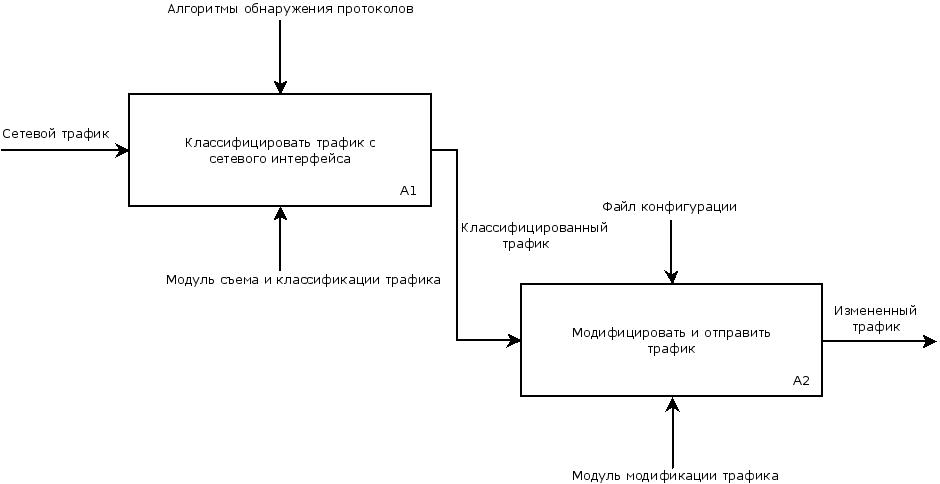
\includegraphics[scale=0.5]{pictures/idef0_schema}
\caption{Схема IDEF0}
\label{pic:idef0_schema}
\end{figure}

Система состоит из двух главных модулей:
\begin{itemize}
\item модуль съема и классификации трафика;
\item модуль модификации трафика;
\end{itemize}

Функциональные требования для модуля съема трафика:
\begin{itemize}
\item съем трафика с сетевого интерфейса;
\item определение класса трафика, используя алгоритмы обнаружения;
\item подсчет статистики по каждому классу трафика;
\end{itemize}

Функциональные требования для модуля модификации трафика:
\begin{itemize}
\item добавление MPLS метки;
\item тегирование VLAN;
\item блокировка нежелательного трафика;
\item отправка трафика в соответствующий порт;
\end{itemize}

\section{Диаграмма состояний разрабатываемого сервиса}
На рисунке~\ref{pic:state_diagram} показана диаграмма состояний сервиса с момента запуска и вплоть до получения сигнала о завершении.
\begin{figure}[h]
\centering
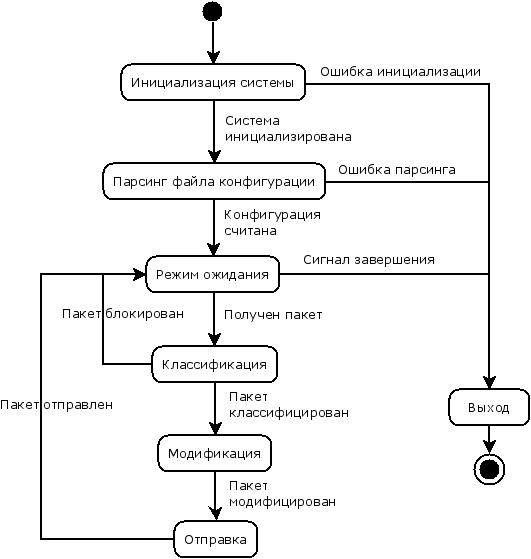
\includegraphics[scale=0.6]{pictures/state_diagram}
\caption{Диаграмма состояний сервиса}
\label{pic:state_diagram}
\end{figure}

В момент инициализации происходит выделение необходимого количества памяти под входные и выходные буфера, инициализация сетевых интерфейсов, привязка потоков к конкретным ядрам процессора. Далее выполняется считывание файла конфигурации, структура которого описана ниже. После выполнения этих операций сервис переходит в режим ожидания, в котором выполняется опрос сетевой карты на предмет появления новых пакетов. Каждый новый пакет проходит классификацию и, если для заданного класса трафика не предусмотрена блокировка, модификацию с последующей отправкой в нужный порт.

\section{Архитектура разрабатываемого сервиса}
На рисунке~\ref{pic:concept_schema} представлена архитектура сервиса на примере обработки трафика с двух сетевых интерфейсов.
\begin{figure}[h]
\centering
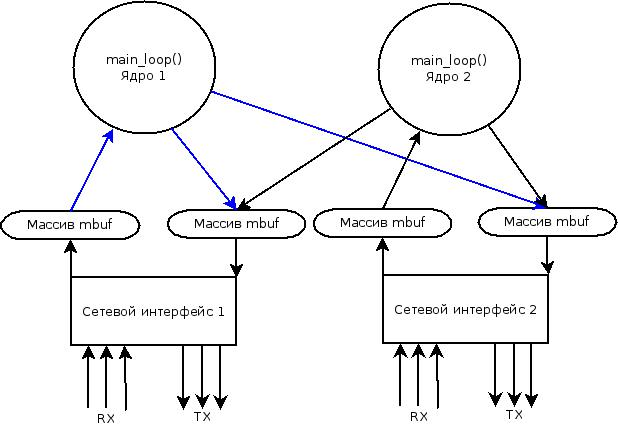
\includegraphics[scale=0.6]{pictures/concept_schema}
\caption{Архитектура сервиса}
\label{pic:concept_schema}
\end{figure}

Пакеты поступают на RX очереди сетевой карты. Количество очередей зависит от самой сетевой карты, но в данной работе используется одна RX очередь. Далее полученные пакеты сохраняются (через DMA) в массив структур mbuf, описанных в DPDK.

При запуске сервиса каждому сетевому интерфейсу назначается ядро, на котором запускается главный цикл обработки, таким образом одну сетевую карту обслуживает одно ядро. Случай, когда разные ядра обслуживают разные RX очереди одной сетевой карты в данной работе не рассматривается.

В главном цикле вычитываются пакеты из массива структур, производится их обработка, а затем они помещаются  в выходной массив структур mbuf нужного интерфейса. Промежуточный массив нужен для того, чтобы не вызывать часто API для отправки данных с сетевой карты, так как это снижает производительность. Вместо этого данные помещаются в буфер, а затем, с некоторой периодичностью, извлекаются и отправляются в TX очередь интерфейса.

\subsection{Выходные очереди}
Количество выходных очередей также зависит от самой сетевой карты, но в данной работе используется одна TX очередь на каждый сетевой интерфейс.

К входному массиву mbuf происходит обращение только из одного ядра, поэтому обеспечивать защищенность этого ресурса не требуется. С выходным массивом все иначе - несколько ядер одновременно могут обращаться к нему, поэтому требуется использовать какой-то подход, гарантирующий безопасность этого ресурса.

Мьютексы, семафоры и другие примитивы синхронизации, требующие блокировки, в данной работе не используются, так как вносят задержку в обработку трафика, тем самым понижая производительность.

Еще одним подходом является разделение данных по ядрам. Именно он применен в данной работе для организации выходного массива mbuf. Для этого создается матрица, число строк которой равно числу ядер в системе, а число столбцов - количеству сетевых интерфейсов (рисунок~\ref{pic:mbuf_matrix}). Элементом такой матрицы является массив mbuf. Каждый раз, когда требуется записать/считать данные в/из выходного буфера, из матрицы извлекается элемент с индексом [номер ядра][номер порта] и дальнейшая работа производится с ним. Такой подход не требует дополнительных действий по обеспечению безопасности, т.к. каждое ядро использует собственную переменную.
\begin{figure}
\centering
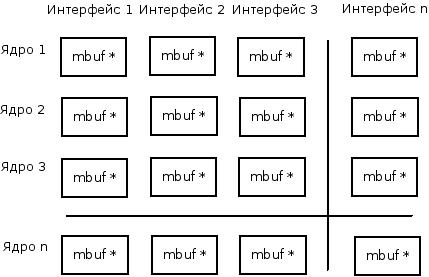
\includegraphics[scale=0.6]{pictures/mbuf_matrix}
\caption{Матрица массивов mbuf}
\label{pic:mbuf_matrix}
\end{figure}

\subsection{Статистика}
Разрабатываемый сервис должен вести статистику по общему количеству полученных и отправленных пакетов, а также статистику по каждому поддерживаемому протоколу.

Общую статистику можно получить через DPDK, используя функцию rte\_eth\_stats\_get(), которой в качестве параметров передается номер порта и структура для заполнения. Сам подсчет реализуется драйвером соответствующей карты.

Статистику по каждому протоколу необходимо реализовывать вручную. Простой способ - это хранить счетчик для каждого типа протокола и, при обнаружении соответствующего пакета, увеличивать его. Так как обновление счетчика производится с разных ядер, требуется защита переменной. Здесь, как и в случае с выходным буфером, используется массив счетчиков (рисунок~\ref{pic:counters}). Полная статистика по конкретному протоколу вычисляется как сумма счетчиков на каждом ядре.
\begin{figure}
\centering
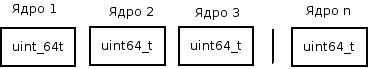
\includegraphics[scale=0.6]{pictures/counters}
\caption{Массив счетчиков}
\label{pic:counters}
\end{figure}

Подход с разделением данных по ядрам имеет скрытую угрозу производительности. Связано это с организацией памяти современных компьютеров, а именно с кэшом. Обычно, размер линейки кэша 64 байта. Допустим, мы используем счетчики размером 8 байт, то есть в одну линейку укладывается 8 таких счетчиков. Изменение хотя бы одного счетчика приводит к инвалидации и обновлению всей линейки памяти, а если такая линейка присутствует в кэше других ядер, то и к синхронизации с ними.

Вся работа по обеспечению когерентности кэшей выполняется протоколом MESI на уровне процессора. Если одинаковые данные присутствуют в кэшах разных ядер, то при их модификации шлется RFO как сигнал о том, что данные больше не действительны и требуется обновить их. Многочисленные запросы RFO опасны так же, как промахи в кэш, так как сильно сказываются на производительности приложения.

Для решения этой проблемы в рамках данной работы используется стратегия выравнивания данных по размеру линейки кэша. Основная идея заключается в том, что в одну линейку помещают только одно изменяемое значение. В результате такая запись будет присутствовать в кэше только того ядра, который с ней работает, что полностью исключает возникновение RFO и повышает производительность.

\section{Поддерживаемые протоколы}
Детальное описание каждого из протоколов, поддерживаемых сервисом, выходит за рамки работы. Ниже приведены лишь их структуры и алгоритмы обнаружения.

\subsection{HTTP}
Обмен сообщениями при использовании HTTP идет по схеме "запрос-ответ". Каждое HTTP-сообщение имеет структуру, приведенную в таблице~\ref{tbl:http_structure}.
\begin{table}
\centering
\caption{Структура HTTP}
\label{tbl:http_structure}
\begin{tabular} {| c |} 
\hline
Стартовая строка\\
\hline
Заголовки\\
\hline
Пустая строка\\
\hline
Тело сообщения\\
\hline
\end{tabular}
\end{table}

Заголовки и тело сообщения могут отсутствовать, но стартовая строка является обязательной, так как указывает на тип запроса/ответа. Запрос отправляется в формате: "тип\_запроса адрес версия\_протокола". Ответ имеет формат: "версия\_протокола код\_возврата пояснения".

Список запросов, согласно~\cite{http_rfc}: OPTIONS, GET, HEAD, POST, PUT, DELETE, TRACE, CONNECT.

Пример запроса:
\begin{lstlisting}
GET HTTP://server/path/test.html HTTP/1.1
\end{lstlisting}


В рамках данной работы поддерживается только HTTP версии 1.1. Проанализировав структуру HTTP, был разработан простой протокол обнаружения, основанный только на типах запросов и версии протокола. Блок-схема приведена на рисунке~\ref{pic:http_alg}.
\begin{figure}
\centering
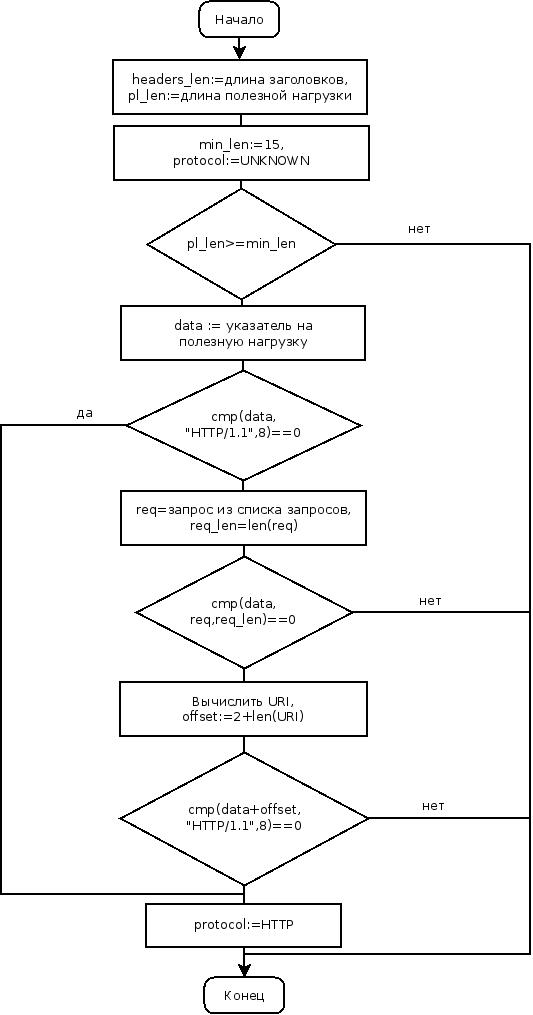
\includegraphics[scale=0.5]{pictures/http_alg}
\caption{Алгоритм обнаружения HTTP}
\label{pic:http_alg}
\end{figure}

\subsection{SIP}
Сообщения протокола SIP представляют собой последовательности текстовых строк (запросы и ответы). Структура и синтаксис идентичны используемым в протоколе HTTP.

Стартовая строка - начальная строка любого SIP-сообщения. Если сообщение является запросом, в ней указывается тип запроса, адресат и номер версии протокола. Если сообщение является ответом - указывается номер версии, тип ответа и короткая расшифровка.

Заголовки сообщений содержат информацию, необходимую для обработки сообщения.

Тело сообщения содержит описание сеансов связи. Не все запросы содержат тело (например, BYE).

Список запросов, согласно~\cite{sip_rfc}: INVITE, ACK, BYE, CANCEL, REGISTER, OPTIONS, PRACK, SUBSCRIBE, NOTIFY, PUBLISH, INFO, REFER, MESSAGE, UPDATE.

Пример запроса:
\begin{lstlisting}
INVITE sip:nikolia@example.ru SIP/2.0
\end{lstlisting}

Проанализировав структуру протокола SIP, был разработан алгоритм обнаружения, блок-схема которого приведена на рисунке~\ref{pic:sip_alg}.
\begin{figure}
\centering
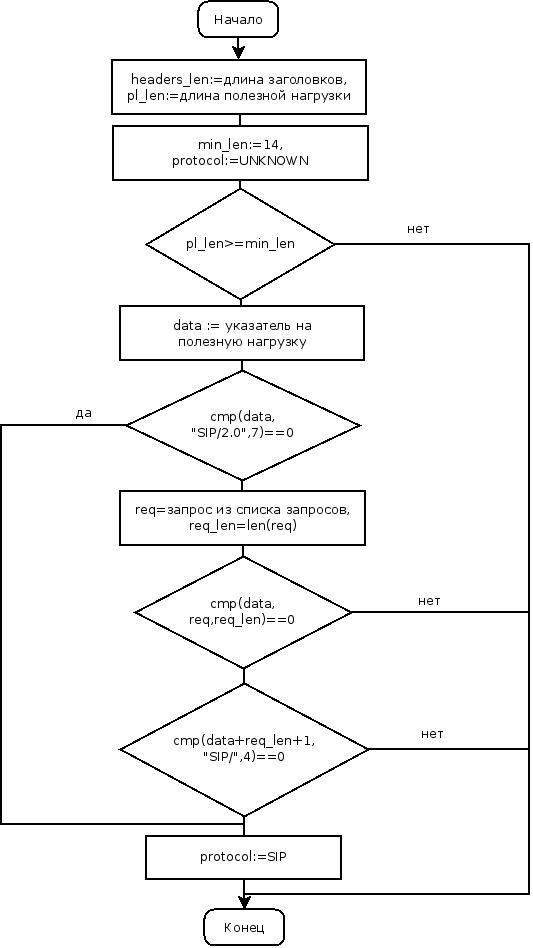
\includegraphics[scale=0.6]{pictures/sip_alg}
\caption{Алгоритм обнаружения SIP}
\label{pic:sip_alg}
\end{figure}

\subsection{RTSP}
По синтаксису и операциям протокол RTSP похож на HTTP, хотя есть и ряд отличий, например в случае RTSP и сервер и клиент могут генерировать запросы.

Запрос на сервер посылается в текстовом виде в формате: "тип\_запроса абсолютный\_адрес контент версия\_протокола". Вместе с запросом могут быть переданы дополнительные служебные поля (на новых строчках запроса). Ответ посылается также в текстовом виде и содержит номер версии, тип ответа и короткую расшифровку.

Список запросов, согласно~\cite{rtsp_rfc}: DESCRIBE, OPTIONS, PLAY, PAUSE, RECORD, REDIRECT, SETUP, ANNOUNCE, GET\_PARAMETER, SET\_PARAMETER, TEARDOWN.

Пример запроса:
\begin{lstlisting}
PLAY RTSP://server/path/test.mpg RTSP/1.0
\end{lstlisting}

Проанализировав структуру протокола RTSP, был разработан алгоритм обнаружения, блок-схема которого приведена на рисунке~\ref{pic:rtsp_alg}.
\begin{figure}
\centering
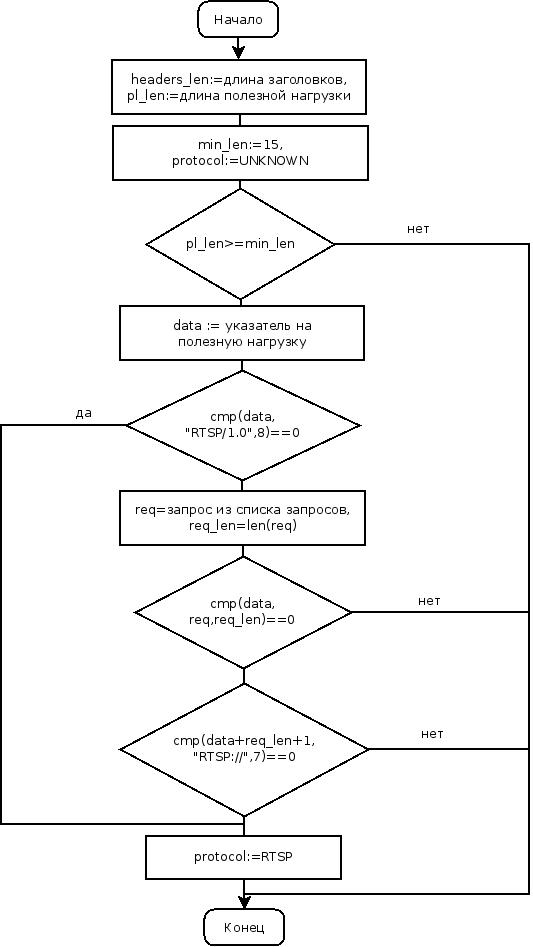
\includegraphics[scale=0.6]{pictures/rtsp_alg}
\caption{Алгоритм обнаружения RTSP}
\label{pic:rtsp_alg}
\end{figure}

\subsection{RTP}
Структура пакета RTP, согласно~\cite{rtp_rfc}, приведена в таблице~\ref{tbl:rtp_structure}.
\begin{table}
\centering
\caption{Структура RTP}
\label{tbl:rtp_structure}
\begin{tabular} {| c | c | c | c | c | c | c | c |} 
\hline
+Биты & 0-1 & 2 & 3 & 4-7 & 8 & 9-15 & 16-31\\
\hline
0 & Ver. & P & X & CC & M & PT & Порядковый номер\\
\hline
32 & \multicolumn{7}{ c |}{Метка времени}\\
\hline
64 & \multicolumn{7}{ c |}{SSRC-идентификатор}\\
\hline
96, если & \multicolumn{7}{ c |}{[CSRC-идентификаторы]}\\
CC>0 & \multicolumn{7}{ c |}{}\\
\hline
96+(CCx32), & \multicolumn{6}{ c |}{[Заголовок расширения -} & [Заголовок расширения - количество\\
если X=1 & \multicolumn{6}{ c |}{определенное профилем значение]} & блоков данных по 32 бита(EHL)]\\
\hline
96+ & \multicolumn{7}{ c |}{[Заголовок расширения - блоки данных]}\\
(CCx32)+32 & \multicolumn{7}{ c |}{}\\
\hline
96+(CCx32) & \multicolumn{7}{ c |}{}\\
+X* & \multicolumn{7}{ c |}{Данные}\\
(32+32xEHL) & \multicolumn{7}{ c|}{}\\
\hline
если P=1 & \multicolumn{6}{ c |}{Выравнивание} & L\\
\hline
\end{tabular}
\end{table}

Ver (2 бита) указывает версию протокола, текущая версия 2.

P (1 бит) используется в случаях, когда RTP-пакет дополняется пустыми байтами на конце.

X (1 бит) используется для указания расширений протокола, задействованных в пакете.

CC (4 бита) содержит количество CSRC-идентификаторов, следующих за постоянным заголовком.

M (1 бит) используется на уровне приложения и определяется профилем, если поле установлено, то данные пакета имеют какое-то особое значение для приложения.

PT (7 бит) указывает формат полезной нагрузки и определяет ее интерпретацию приложением, допустимые значения: 0-34, 96-127.

SSRC (64-95 бита) указывает источник синхронизации, не может быт равным 0.

EHL (Extension Header Length) - количество 32-битных слов в блоке данных расширения заголовка.

L - последний байт в пакете, определяющий длину области заполнения в байтах (используется для выравнивания в последнем пакете).

Проанализировав структуру протокола RTP, был разработан алгоритм обнаружения, блок-схема которого приведена на рисунке~\ref{pic:rtp_alg}.
\begin{figure}
\centering
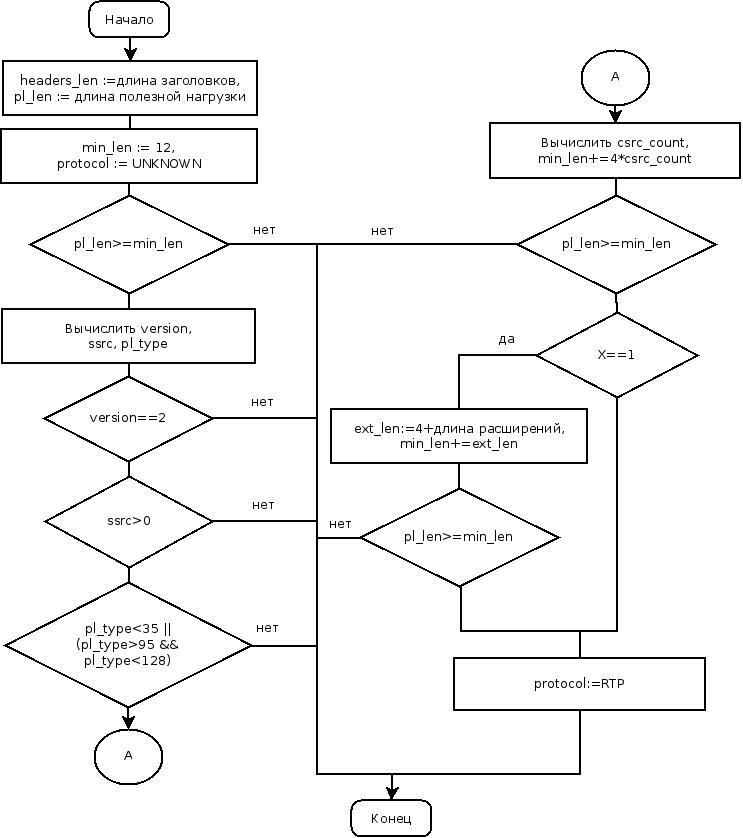
\includegraphics[scale=0.6]{pictures/rtp_alg}
\caption{Алгоритм обнаружения RTP}
\label{pic:rtp_alg}
\end{figure}


\section{Конфигурационный файл}
\subsection{Структура}
Конфигурационный файл используется для того, чтобы определить поведение сервиса при обнаружении поддерживаемых протоколов. В нем описываются порты, протоколы, которые необходимо детектировать на этом порте и набор действий, выполняемый при обнаружении.

Сам файл задается в текстовом виде и имеет следующую структуру:
\begin{center}
номер\_порта,протокол : список действий;
\end{center}

Основные особенности:
\begin{itemize}
\item между составными частями допускается любое количество пробелов;
\item список действий не может быть пустым;
\item протокол должен быть одним из списка поддерживаемых сервисом;
\item пакеты неописанных протоколов по умолчанию блокируются;
\item номер порта указывается в численном виде;
\item протокол задается большими английскими буквами;
\item UNKNOWN используется для неподдерживаемых протоколов;
\end{itemize}

\subsection{Действия и допустимые значения}
Все параметры действий указываются в круглых скобках и задаются в десятичной системе счисления. Описание действия всегда оканчивается символом ";". Порядок объявления в списке действий зависит от самого действия и описан ниже.

\paragraph{DROP}

Не имеет параметров, используется для явной блокировки определенного типа трафика. В списке действий должно располагаться первым, остальные действия, если присутствуют, не выполняются.

Пример описания:
\begin{lstlisting}
1,SIP : DROP;
\end{lstlisting}

\paragraph{OUTPUT}

В качестве параметра указывается номер выходного порта. Может использоваться несколько раз, например для реализации широковещательной рассылки. В списке действий должно быть последним действием.

Пример описания:
\begin{lstlisting}
1,SIP : OUTPUT(2);
\end{lstlisting}

\paragraph{PUSH-VLAN}

В качестве параметров указывается набор из 4 чисел, разделенных запятой, состоящий из:
\begin{itemize}
\item TPID - 0x8100 для тегирования 802.1Q и 0x88A8 для 802.1AD;
\item PCP - ограничен размером поля (3 бита);
\item CFI - ограничен размером поля (1 бит);
\item VID - ограничен размером поля (12 бит), а также зарезервированными значениями;
\end{itemize}

Может использоваться несколько раз, например для реализации QinQ. В списке действий должно располагаться до действия OUTPUT.

Пример описания:
\begin{lstlisting}
1,SIP : PUSH-VLAN(33024, 3, 1, 100);
\end{lstlisting}

\paragraph{PUSH-MPLS}

В качестве параметров указывается набор из 4 чисел, разделенных запятой, состоящий из:
\begin{itemize}
\item LABEL - ограничен размером поля (20 бит);
\item CoS - ограничен размером поля (3 бита);
\item S - ограничен размером поля (1 бит);
\item TTL - ограничен размером поля (8 бит);
\end{itemize}

Может использоваться несколько раз, например для создания стека MPLS меток. В списке действий должно располагаться до действия OUTPUT.

Пример использования:
\begin{lstlisting}
1,SIP : PUSH-MPLS(100, 3, 1, 64);
\end{lstlisting}

\paragraph{Выводы}

В рамках данного раздела была разработана схема IDEF0 и диаграмма состояний сервиса. Также были изучены структуры протоколов, поддерживаемых сервисом, и на их основе разработаны алгоритмы обнаружения с блок-схемами. В конце раздела описана структура конфигурационного файла, допустимые действия и их параметры.
